\subsection{Chapter 17 - Electric potential}

\subsubsection{Overview}\label{chapter:potential}

In this chapter, we develop the concept of electric potential energy and electric potential. This will allow us to describe the motion of charges using energy instead of forces. We will also introduce the capacitor, a common circuit component that is used to store charge.

\begin{framed}
\textbf{Learning Objectives}\\
\begin{itemize}
\item Understand the difference between electrical potential energy and electric potential.
\item Understand how to calculate stored electrostatic potential energy.
\item Understand how to calculate the electric potential difference between two points near a point charge or a distribution of charges.
\item Understand how to use electric potential to determine electrical potential energy.
\item Understand how to determine electric potential from electric field.
\item Understand how to determine electric field from electric potential.
\item Understand how to model a capacitor.
\end{itemize}
\end{framed}

\begin{framed}
\textbf{Think About It}\\
A proton and an electron are both accelerated by the $110 {\rm V}$ electric potential difference from your outlet. Which particle has the highest speed?

\begin{enumerate}
\item The proton.
\item The electron.
\item They will have the same speed, since they were accelerated by the same potential difference.
\end{enumerate}

\begin{framed}
\textbf{Answer}\\
\begin{enumerate}[resume]
\item
\end{enumerate}
\end{framed}
\end{framed}

\subsubsection{Electric potential energy}\label{sec:potential:potentialdefinition}

\begin{framed}
\textbf{Review}\\
\begin{itemize}
\item Section~\ref{sec:potentialecons:conservative} on conservative forces.
\item Section~\ref{sec:gravity:potentialenergy} on the derivation of gravitational potential energy.
\end{itemize}
\end{framed}

Mathematically, Coulomb's Law for the electric force is identical to Newton's Universal Theory of Gravity for the gravitational force. The electric force is thus conservative, and the work done by the electric force on a charge, $q$, when the charge moves from position $A$ in space to some other position $B$, cannot depend on the path taken. Since the work done by the electric force only depends on the location of the initial ($A$) and final ($B$) positions, we can define an electrical potential energy function, $U(\vec r)$, that depends on position, $\vec r$. The work done by the electric force, $\vec F^E$,  on a charge in going from position $A$ (defined by position vector, $\vec r_A$), to position $B$ (defined by position vector, $\vec r_B$), can be written as:
\begin{equation}
\label{eqn:potential:potentialwork}
W=\int_A^B \vec F^E\cdot d\vec r=-\Delta U=-\left[ U(\vec r_B)-U(\vec r_A) \right]
\end{equation}
In order to determine the function, $U(\vec r)$, we can choose a path over which the integral for work is easy to calculate. Consider a point charge, $+Q$, that exerts an electric force on another charge, $+q$, as in Figure~\ref{fig:potential:potential}. We will calculate work done by the electric force as it moves $+q$ from a distance $r_A$ to a distance $r_B$ from the centre of $+Q$.

\begin{figure}[!htbp]
\centering
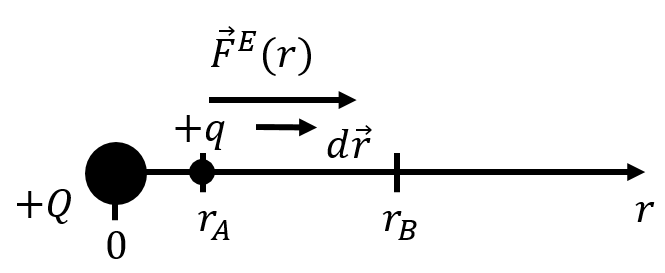
\includegraphics[width=0.5\linewidth]{files/potential-891c4cc60bcc90cd78ce4c04667f85f1.png}
\caption[]{Calculating the work done on a charge $+q$ by the electric force exerted by charge $+Q$ when charge $+q$ moves from a distance $r_A$ to a distance $r_B$ from the centre of charge $+Q$.}
\label{fig:potential:potential}
\end{figure}

Placing $+Q$ at the origin of a coordinate system, the force exerted on $+q$, when it is located at position $\vec r$, is given by:
\begin{equation}
\vec F^E=k\frac{Qq}{r^2}\hat r
\end{equation}
The work done by the electric force when $+q$ moves from $r_A$ to $r_B$ is given by:
\begin{equation}
W&=\int_A^B \vec F^E\cdot d\vec r=\int_{\vec r_A}^{\vec r_B} \left(k\frac{Qq}{r^2}\hat r\right)\cdot d\vec r=kQq \int_{r_A}^{r_B} \frac{1}{r^2}dr\\
&=kQq \left[\frac{-1}{r} \right]_{r_A}^{r_B}=-\left(\frac{kQq}{r_B}-\frac{kQq}{r_A}\right)
\end{equation}
where we noted that, since $\vec F^E$ and $d\vec r$ are parallel, their scalar product is simply the product of their magnitudes. By comparing with (\ref{eqn:potential:potentialwork}), we can identify the potential energy, $U(\vec r)$, of a charge, $+q$, located at a relative position, $\vec r$, from a point charge, $+Q$, as:
\begin{equation}
\boxed{U(\vec r)=\frac{kQq}{r}+C}
\end{equation}
where the potential energy is only defined up to some constant, $C$, which cancels when we take the difference in potential energy between two positions. Note that this is very similar to the function for the gravitational potential energy of a mass, $m$, a distance, $r$, from a mass, $M$ (see Section~\ref{sec:gravity:potentialenergy}).

The potential energy function that we derived above remains the same if one or both of the charges change sign. The only difference in the derivation would be that the direction of the force, $\vec F^E$, could change. For example, a positive charge, $+q$, near a negative charge, $-Q$, would have negative electric potential energy with the choice $C=0$, in exact analogy with gravity.

\paragraph{Electrostatic potential energy}

When we hold two positive charges together a distance, $r$, apart, we need to exert a force on the charges in order to keep the charges in place (as they repel each other). If we release the charges, they will move apart from each other until all of the stored electric potential energy is converted into kinetic energy. The energy that was originally stored in this ``system'' of two charges is called ``electrostatic potential energy''. In this section, we show how to model the energy stored in a collection of point charges.

Consider a single positive charge, $q_1$, located at the origin of empty space. Since there are no other charges present, it does not ``cost'' us any energy to place that charge there - we do not need to do any work. If we now bring in a second positive charge, $q_2$, and place it a distance, $r_{12}$, from $q_1$ (Figure~\ref{fig:potential:electrostaticenergy}), we will need to do work since $q_1$ exerts a force on $q_2$. We define zero potential energy to be at infinity, which means choosing $C=0$ for electric potential energy. The work, $W_{q2}$, that we must do on $q_2$ to bring it from infinity to a distance, $r_{12}$, from $q_1$ is given by the corresponding change in potential energy of $q_2$:
\begin{equation}
W_{q2}=\Delta U=U_{final}-U_{initial}=k\frac{q_1q_2}{r_{12}}-0=k\frac{q_1q_2}{r_{12}}
\end{equation}
Note that the work is done by us (not by the electric field), so it has the same sign as the change in potential energy (we must do positive work to increase potential energy). The work that we did corresponds to the same amount of electrostatic potential energy stored in this arrangement of two charges (the only source of that stored electrostatic potential energy is the work that we did on the charge $q_2$).

\begin{figure}[!htbp]
\centering
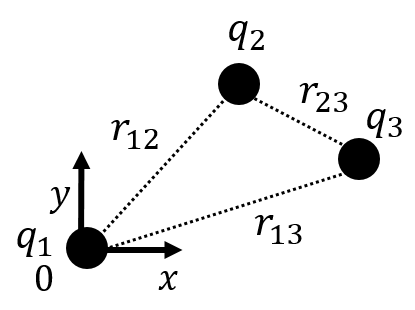
\includegraphics[width=0.3\linewidth]{files/electrostaticenergy-89ace4c8bca7c6e872fcfeae1c265bc3.png}
\caption[]{Three positive charges arranged together will store a certain amount of electrostatic potential energy.}
\label{fig:potential:electrostaticenergy}
\end{figure}

Now, we bring in a third positive charge, $q_3$, also from infinitely far away, as illustrated in Figure~\ref{fig:potential:electrostaticenergy}. In order to bring in $q_3$, we need to do work against the forces exerted by both $q_1$ and $q_2$. Suppose that we place $q_3$ a distance $r_{13}$ from $q_1$ and $r_{23}$ from $q_2$. Then, the amount of work done by us to bring in $q_3$ is given by:
\begin{equation}
W_{q3}=k\frac{q_1q_3}{r_{13}}+k\frac{q_2q_3}{r_{23}}
\end{equation}
and the total electrostatic energy stored in the system of three charges is given by the sum of the work done to place $q_2$ and the work done to place $q_1$:
\begin{equation}
E = W_{q1}+W_{q2}+W_{q3}=0+k\frac{q_1q_2}{r_{12}}+k\frac{q_1q_3}{r_{13}}+k\frac{q_2q_3}{r_{23}}
\end{equation}
If we have any number of charges (positive and negative), we can always calculate the stored electrostatic energy by proceeding in a similar fashion.

\begin{framed}
\textbf{Checkpoint}\\
Four charges of varying magnitude are fixed in position. If the electric potential energy stored in the system were to be calculated as above, how many terms would be in the sum?

\begin{enumerate}
\item Four.
\item Two.
\item One.
\item Six.
\end{enumerate}

\begin{framed}
\textbf{Answer}\\
\begin{enumerate}[resume]
\item
\end{enumerate}
\end{framed}
\end{framed}

\subsubsection{Electric potential}

As you recall, we defined the \textbf{electric field}, $\vec E(\vec r)$, to be the \textbf{electric force per unit charge}. By defining an electric field everywhere in space, we were able to easily determine the force on any test charge, $q$, whether the test charge is positive or negative (since the sign of $q$ will change the direction of the force vector, $q\vec E$):
\begin{equation}
\vec E(\vec r) &= \frac{\vec F^E(\vec r)}{q}\\
\therefore \vec F^E(\vec r)&=q\vec E(\vec r)
\end{equation}
Similarly, we define the \textbf{electric potential}, $V(\vec r)$, to be the \textbf{electric potential energy per unit charge}. This allows us to define electric potential, $V(\vec r)$, everywhere in space, and then determine the potential energy of a specific charge, $q$, by simply multiplying $q$ with the electric potential at that position in space.
\begin{equation}
V(\vec r) &= \frac{ U(\vec r)}{q}\\
\therefore U(\vec r)&= q V(\vec r)
\end{equation}
The S.I. unit for electric potential is the ``volt'' (V). Electric potential, $V(\vec r)$, is a scalar field whose value is ``the electric potential'' at that position in space. Say that the electric potential at a position in space is  $V=10 {\rm V}$. The above formula tells us that a positive charge $q=1 {\rm C}$, located at that position, will have a potential energy of $U=10 {\rm J}$. Similarly, a negative charge, $q= -1 {\rm C}$, will have negative potential energy, $U= -10 {\rm J}$, at the same location.

Since only \textit{differences} in potential energy are physically meaningful, \textbf{only changes in electrical potential are physically meaningful}. A difference in electric potential is commonly called a ``voltage''. One often makes a clear choice of where the electric potential is zero (typically the ground, or infinitely far away), so that the term voltage is used to describe potential, $V$, instead of difference in potential, $\Delta V$; this should only be done when it is clear where the location of zero electric potential is defined.

We can describe a free-falling mass by stating that the mass moves from a region where it has high gravitational potential energy to a region of lower gravitational potential energy under the influence of gravity (the force associated with a potential energy always acts in the direction to decreases potential energy). The same is true for electrical potential energy: \textbf{charges will always experience a force in a direction to decrease their electrical potential energy}. However, positive charges will experience a force driving them from regions of high electric potential to regions of low electric potential, whereas negative charges will experience a force driving them from regions of low electric potential to regions of higher electric potential. This is because, for negative charges, the change in potential energy associated with moving through space, $\Delta U$, will be the negative of the corresponding change in electric potential, $\Delta U=q\Delta V$, since the charge, $q$, is negative.

% TODO: kind of confusing

\begin{framed}
\textbf{Checkpoint}\\
Electric potential increases along the $x$ axis. A proton and an electron are placed at rest at the origin; in which direction do the charges move when released?\}

\begin{enumerate}
\item the proton moves towards negative $x$, while the electron moves towards positive $x$.
\item the proton moves towards positive $x$, while the electron moves towards negative $x$.
\item the proton and electron move towards negative $x$.
\item the proton and electron move towards positive $x$.
\end{enumerate}

\begin{framed}
\textbf{Answer}\\
\begin{enumerate}
\item
\end{enumerate}
\end{framed}
\end{framed}

If the only force exerted on a particle is the electric force, and the particle moves in space such that the electric potential changes by $\Delta V$, we can use conservation of energy to determine the corresponding change in kinetic energy of the particle:
\begin{equation}
\Delta E &= \Delta U + \Delta K = 0\\
\Delta U &= q\Delta V\\
\end{equation}
\begin{equation}
\boxed{\therefore \Delta K = -q \Delta V}
\end{equation}
where $\Delta E$ is the change in total mechanical energy of the particle, which is zero when energy is conserved. The kinetic energy of a positive particle increases if the particle moves from a region of high potential to a region of low potential (as $\Delta V$ would be negative and $q$ is positive), and vice versa for a negative particle. This makes sense, since a positive and negative particle feel forces in opposite directions.

In order to describe the energies of particles such as electrons, it is convenient to use a different unit of energy than the Joule, so that the quantities involved are not orders of magnitude smaller than 1. A common choice is the ``electron volt'', eV\}. One electron volt corresponds to the energy acquired by a particle with a charge of $e$ (the charge of the electron) when it is accelerated by a potential difference of $1 {\rm V}$:
\begin{equation}
\Delta E &= q\Delta V\\
1 {\rm eV}&=(e)(1 {\rm V})=1.6\times 10^{-19} {\rm J}
\end{equation}
An electron that has accelerated from rest across a region with a $150 {\rm V}$ potential difference across it will have a kinetic of $150 {\rm eV}=2.4\times 10^{ -17} {\rm J}$. As you can see, it is easier to describe the energy of an electron in electron volts than Joules.

\begin{framed}
\textbf{Checkpoint}\\
A particle moves from an electric potential of $-260 {\rm V}$ to an electric potential of $-600 {\rm V}$ and loses kinetic energy. What is the charge of this particle?

\begin{enumerate}
\item Neutral.
\item It could have a positive or a negative charge.
\item Positive.
\item Negative.
\end{enumerate}

\begin{framed}
\textbf{Answer}\\
\begin{enumerate}[resume]
\item
\end{enumerate}
\end{framed}
\end{framed}

\begin{framed}
\textbf{Josh's Thoughts}\\
It is often useful in physics to take previously learned concepts and compare them to new ones, in this case, gravitational potential energy and electric potential energy can be compared to help understand the physical meaning of electric potential.

Suppose that an object with a large mass, $M$, is sitting in space. Now place an object of a much smaller mass, $m$, at any distance, $r$, from the centre of $M$. The gravitational potential energy of the small mass is given by the following formula:
\begin{equation}
U_g&=\frac{GMm}{r}
\end{equation}
Which is very similar to the formula for electrical potential energy:
\begin{equation}
U(\vec r)&=\frac{kQq}{r}
\end{equation}
Now, if we were to remove the mass $m$ from its position, we would no longer have an object with gravitational potential energy. However, we could still describe the gravitational potential for the point, $r$, which would result in gravitational potential energy when any mass $m$ is placed there. This is the gravitational equivalent to electric potential, and can be defined as:
\begin{equation}
V_g&=\frac{U_g}{m}
\end{equation}
which is also very similar to the formula for electric potential:
\begin{equation}
V_E&=\frac{U_E}{q}
\end{equation}
This comparison is illustrated in Figure~\ref{fig:potential:gravvselec}.

\begin{figure}[!htbp]
\centering
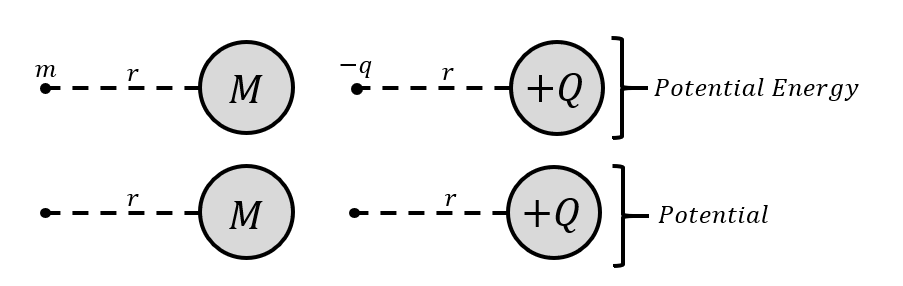
\includegraphics[width=0.6\linewidth]{files/gravvselec-a557143162401d4b8e45aadb66017e48.png}
\caption[]{Gravitational potential energy and gravitational potential (left) next to its electrical analogue (right).}
\label{fig:potential:gravvselec}
\end{figure}
\end{framed}

\begin{framed}
\textbf{Example 17.1}\\
A proton and an electron move from a region of space where the electric potential is $20 {\rm V}$ to a region of space where the electric potential is $10 {\rm V}$. If the electric force is the only force exerted on the particles, what can you say about their change in speed?

\begin{framed}
\textbf{Solution}\\
The two particles move from a region of space where the electric potential is $20 {\rm V}$ to a region of space where the electric potential is $10 {\rm V}$. The change in electric potential experienced by the particles is thus:
\begin{equation}
\Delta V = V_{final}-V_{initial}=(10 {\rm V})-(20 {\rm V})=-10 {\rm V}
\end{equation}
and we take the opportunity to emphasize that one should be very careful with signs when using potential. The change in potential energy of the proton, with charge $q=+e$, is thus:
\begin{equation}
\Delta U_p=q\Delta V = (+e)(-10 {\rm V})=-10 {\rm eV}
\end{equation}
The potential energy of the proton thus decreases by $10 {\rm eV}$ (which you can easily convert to Joules). Since we are told that no other force is exerted on the particle, the total mechanical energy of the particle (kinetic plus potential energies) must be constant. Thus, if the potential energy decreased, then the kinetic energy of the proton has increased by the same amount, and \textbf{the proton's speed increases}.

The change in potential energy of the electron, with charge $q= -e$, is thus:
\begin{equation}
\Delta U_e=q\Delta V = (-e)(-10 {\rm V}) = 10 {\rm eV}
\end{equation}
The potential energy of the electron thus increases by $10 {\rm eV}$. Again, the mechanical energy of the electron is conserved, so that an increase in potential energy results in the same decrease in kinetic energy and \textbf{the electron's speed decreases}.

\textbf{Discussion:} By using the electric potential, $V$, we modelled the change in electric potential energy of a proton and an electron as they both moved from one region of space to another.

We found that when a \textbf{proton moves from a region of high electric potential to a region of lower electric potential, its potential energy decreases}. This is because the proton has a positive charge and a decrease in electric potential will also result in a decrease in potential energy. Since no other forces are exerted on the proton, the proton's kinetic energy must increase. Because the potential energy of the proton decreases, the proton is moving in the same direction as the electric force, and the electric force does positive work on the proton to increase its kinetic energy.

Conversely, we found that when an \textbf{electron moves from a region of high electric potential to a region of lower electric potential, its potential energy increases}. This is because it has a negative charge and a decrease in electrical potential thus results in an increase in potential energy. Since no other forces are exerted on the electron, the electron's kinetic energy must decrease, and the electron slows down. This makes sense, since the force that is exerted on an electron will be in the opposite direction from the force exerted on a proton.
\end{framed}
\end{framed}

\paragraph{Electric potential from electric field}

At the beginning of Section~\ref{sec:potential:potentialdefinition}, we determined the potential energy of a point charge, $q$, in the presence of another point charge, $Q$ (Figure~\ref{fig:potential:potential}). This was done by calculating the work done by the Coulomb (electric) force exerted by charge $Q$ on $q$. We can write the same integral for the work done by the electric force on $q$, but using the electric field, $\vec E$, to write the force:
\begin{equation}
W&=\int_A^B \vec F^E\cdot d\vec r=\int_A^B q \vec E\cdot d\vec r=q \int_A^B  \vec E\cdot d\vec r
\end{equation}
where we recognized that the charge, $q$, is constant and can come out of the integral. The integral that is left is thus the work done by the electric field, $\vec E$, \textit{per unit charge}. In other words, this is the negative change in electric potential:
\begin{equation}
W=q \int_A^B  \vec E\cdot d\vec r=-q\Delta V = -q\left[ V(\vec r_B)-V(\vec r_A) \right]
\end{equation}
\begin{equation}
\boxed{\therefore \Delta V =V(\vec r_B)-V(\vec r_A)=-\int_A^B  \vec E\cdot d\vec r}
\end{equation}
which allows us to easily determine the change in electric potential associated with an electric field. Note that this result is general and does not require the electric field to be that of a point charge, and can be used to determine the electric potential associated with any electric field. We can also specify a function for the potential, up to an arbitrary constant, $C$, (think definite versus indefinite integrals):
\begin{equation}
V(\vec r)=-\int \vec E\cdot d\vec r + C
\end{equation}
The relation between electric potential and electric field is analogous to the relation between electric potential energy and electric force:
\begin{equation}
\Delta V &=V(\vec r_B)-V(\vec r_A)=-\int_A^B  \vec E\cdot d\vec r\\
\Delta U &=U(\vec r_B)-U(\vec r_A)=-\int_A^B  \vec F^E\cdot d\vec r
\end{equation}
as the bottom equation is just $q$ times the first equation. We can think of electric potential being to potential energy what electric field is to electric force. Electric potential and electric field are electric potential energy and electric force, \textit{per unit charge}, respectively.

For a point charge, $Q$, located at the origin, the electric field at some position, $\vec r$, is given by Coulomb's Law:
\begin{equation}
\vec E=\frac{kQ}{r^2}\hat r
\end{equation}
The potential difference between location $A$ (at position $\vec r_A$) and location $B$ (at position $\vec r_B$), as in Figure~\ref{fig:potential:potential}, is given by:
\begin{equation}
\Delta V &=- \int_A^B  \vec E\cdot d\vec r= -\int_{\vec r_A}^{\vec r_B}  \frac{kQ}{r^2}\hat r\cdot d\vec r=-\left(\frac{kQ}{r_B}-\frac{kQ}{r_A}\right)
\end{equation}
and we note that we can write a function for the electric potential, $V(\vec r)$, at a distance $r$ from a point charge, $Q$, as:
\begin{equation}
V(\vec r)=\frac{kQ}{r}+C
\end{equation}
where $C$ is an arbitrary constant. This, of course, is identical to the result that we obtained earlier, for the potential energy of a charge, $q$, a distance, $r$, from $Q$:
\begin{equation}
U(\vec r)=qV(\vec r)=\frac{kQq}{r}+C'
\end{equation}
where the constant, $C'=qC$, does not have any physical impact. Often, as is the case for gravity, one chooses the constant $C=0$. This choice corresponds to defining potential energy to be zero at infinity. Equivalently, this corresponds to choosing infinity to be at an electric potential of $0 {\rm V}$.

\begin{framed}
\textbf{Checkpoint}\\
What causes a positively charged particle to gain speed when it is accelerated through a potential difference?

\begin{enumerate}
\item The particle accelerates because it loses potential energy as it moves from high to low potential.
\item The particle accelerates because it loses potential energy as it moves from low to high potential
\item The particle accelerates because it gains potential energy.
\item The particle accelerates because it moves towards negative charges.
\end{enumerate}

\begin{framed}
\textbf{Answer}\\
\begin{enumerate}
\item
\end{enumerate}
\end{framed}
\end{framed}

\begin{framed}
\textbf{Olivia's Thoughts}\\
Below, I've included a grid you can use to remember how the electric field ($\vec E$), electric force ($\vec F$), electric potential ($V$), and electric potential energy ($U$) relate to one another.

\begin{figure}[!htbp]
\centering
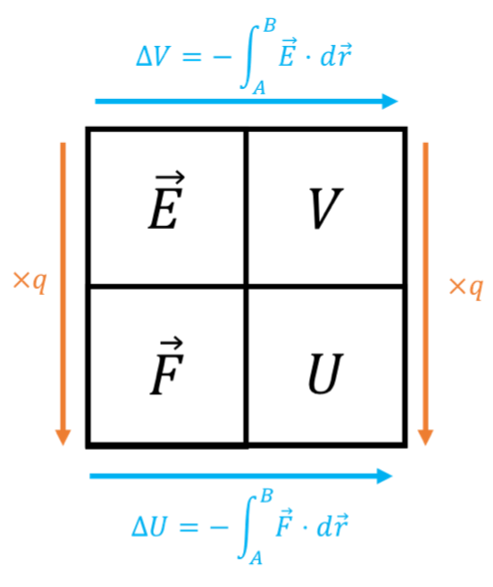
\includegraphics[width=0.4\linewidth]{files/eqn_gridcrop-f3d5ae82cbd9e8f530e5625fd7d75deb.png}
\caption[]{A visual guide showing how to get one formula from another.}
\label{fig:potential:eqn_grid}
\end{figure}

For example, let's say you are given the electric field and want to find the electric potential energy for a charge $q$. You would start at $\vec E$ and follow the operations on the arrows to get to $U$, i.e. you would perform the line integral and then multiply by $q$, or vice versa.

Of course, when you reverse directions (e.g. to go from $U$ to $\vec E$), you have to reverse the operations of the arrows. We will see what the reverse operation of the line integral is in Section~\ref{sec:potential:fieldfrompotential}. Figure~\ref{fig:potential:eqn_grid_point} shows how this grid would be filled out if you were dealing with two point charges, $Q$ and $q$, as we have seen so far in this chapter.

\begin{figure}[!htbp]
\centering
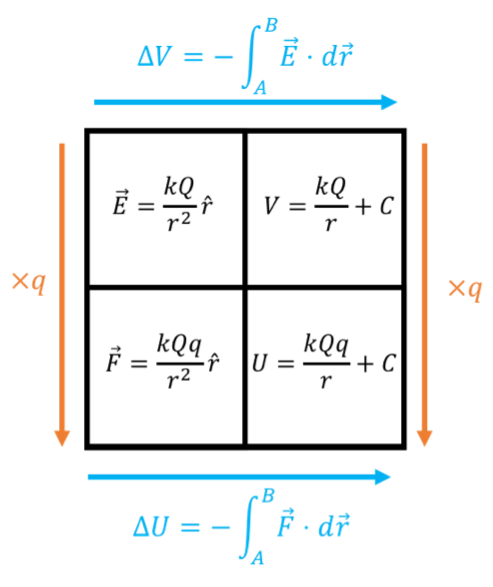
\includegraphics[width=0.4\linewidth]{files/eqn_grid_pointcrop-94d3448ac4141a3f995476c79cd2bb7c.png}
\caption[]{How you would use the guide in the case of a point charge, $Q$, exerting a force on another point charge, $q$.}
\label{fig:potential:eqn_grid_point}
\end{figure}
\end{framed}

\begin{framed}
\textbf{Example 17.2}\\
What is the electric potential at the edge of a hydrogen atom (a distance of $1 \overset{\circ}{\rm A}$ from the proton), if one sets $0 {\rm V}$ at infinity? If an electron is located at a distance of $1 \overset{\circ}{\rm A}$ from the proton, how much energy is required to remove the electron; that is, how much energy is required to ionize the hydrogen atom?

\begin{framed}
\textbf{Solution}\\
We can easily calculate the electric potential, a distance of $1 \overset{\circ}{\rm A}$ from a proton, since this corresponds to the potential from a point charge (with $C=0$):
\begin{equation}
V(\vec r)&=\frac{kQ}{r}\\
&=\frac{(9\times 10^{9} {\rm N\cdot m^2/C^{2}})(1.6\times 10^{-19} {\rm C})}{(1\times 10^{-10} {\rm m})}\\
&=14.4 {\rm V}
\end{equation}
We can calculate the potential energy of the electron (relative to infinity, where the potential is $0 {\rm V}$, since we chose $C=0$):
\begin{equation}
U&=(-e)V\\
&=(-1.6\times 10^{-19} {\rm C})(14.4 {\rm V})=-14.4 {\rm eV}\\
&=-2.3\times 10^{-18} {\rm J}
\end{equation}

where we also expressed the potential energy in electron volts. In order to remove the electron from the hydrogen atom, we must exert a force (do work) until the electron is infinitely far from the proton. At infinity, the potential energy of the electron will be zero (by our choice of $C=0$). When moving the electron from the hydrogen atom to an infinite distance away, we must do positive work to counter the attractive force from the proton. The work that we must do is exactly equal to the change in potential energy of the electron (and equal to the negative of the work done by the force exerted by the proton):
\begin{equation}
W&=\Delta U\\
&=(U_{final}-U_{initial})\\
&=(0 {\rm J}--2.3\times 10^{-18} {\rm J})\\
&=2.3\times 10^{-18} {\rm J}
\end{equation}
The positive work that we must do, exerting a force that is opposite to the electric force, is positive and equal to $2.3\times 10^{ -18} {\rm J}$, or $14.4 {\rm eV}$. If you look up the ionization energy of hydrogen, you will find that it is $13.6 {\rm eV}$, so that this very simplistic model is quite accurate (we could improve the model by adjusting the proton-electron distance so that the potential is $13.6 {\rm V}$).

\textbf{Discussion:} In this example, we determined the electrical potential energy of an electron in a hydrogen atom, and found that it is negative, when potential energy is defined to be zero at infinity. In order to remove the electron from the atom, we must do positive work in order to increase the potential energy of the electron from a negative value to zero (the potential energy at infinity). This is analogous to the work that must be done on a satellite in a gravitationally bound orbit for it to reach escape velocity.
\end{framed}
\end{framed}

\begin{framed}
\textbf{Example 17.3}\\
Two large parallel plates are separated by a distance, $L$. The plates are oppositely charged and carry the same magnitude of charge per unit area, $\sigma$. What is the potential difference between the two plates? Write an expression for the electric potential in the region between the two plates. Assume that the plates are large enough that you can treat them as infinite (that is, neglect what happens near the edges).

\begin{framed}
\textbf{Solution}\\
Figure~\ref{fig:potential:parallelplates} shows a diagram of the two parallel plates with surface charge on them.

\begin{figure}[!htbp]
\centering
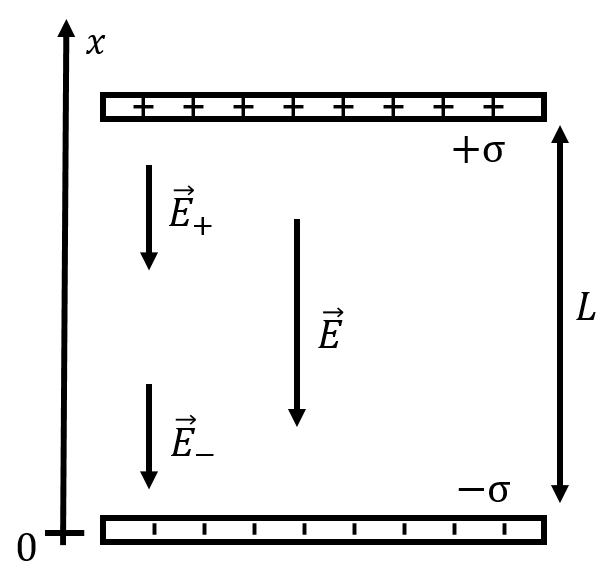
\includegraphics[width=0.3\linewidth]{files/parallelplates-a34555efaf5a4a7e277f17eaeca8f996.png}
\caption[]{Two parallel plates with equal and opposite surface charge densities. In the region between the plates, the electric field is uniform.}
\label{fig:potential:parallelplates}
\end{figure}

We know from the previous chapters that the electric field from the positive plate does not depend on distance from the plate and is given by:
\begin{equation}
\vec E_+=-\frac{\sigma}{2\epsilon_0} \hat x
\end{equation}
if we approximate the plate as being infinitely large. This is a reasonable approximation for most points except those near the edges of the plate, which we ignore. The electric field from the negative plate will have the same magnitude and direction, so that the total electric field, $\vec E$, everywhere between the two parallel plates (as long as we are not near the edges) is given by:
\begin{equation}
\vec E=-\frac{\sigma}{\epsilon_0} \hat x
\end{equation}
Note that the electric field outside the region between the two plates is zero everywhere, as the field from the positive and negative plates point in opposite directions outside the plates and thus cancel (except near the edges of the plates). For example, below the negative plate, the field from the negative plate points in the positive $x$ direction (towards the negative plate), whereas the field from the positive plate points in the negative $x$ direction (away from the positive plate).

We can now determine the potential difference between the two plates, since we know the electric field in that region. Using the coordinate system that is shown, we calculate the potential difference between the positive plate located at $x=L$ and the negative plate located at $x=0$:
\begin{equation}
\Delta V &=V(L)-V(0)\\
&=- \int_0^L  \vec E\cdot d\vec x\\
&=-\int_0^L\frac{-\sigma}{\epsilon_0} \hat x \cdot d\vec x\\
&=\frac{\sigma}{\epsilon_0}\int_0^L dx\\
&=\frac{\sigma}{\epsilon_0}L
\end{equation}
where we recognized that $\hat x$ and $d\vec x$ are parallel. It is very easy to get the wrong sign when calculating potential differences, so be careful!

Since the potential difference, $\Delta V=V(L) -V(0)$, is positive, the plate at $x=L$ is at a higher electric potential than the plate at $x=0$. This makes sense, as a positive charge at rest would move from the positive plate to the negative plate, thus decreasing its potential energy, which corresponds to moving from a region of high electric potential to a region of low electric potential. Conversely, a negative charge at rest would move from the negative plate to the positive plate, decreasing its potential energy, but moving from a region of low electric potential to a region of high electric potential.

In general, if the electric field is constant, the change in potential between two points separated by a distance, $L$, along an axis that is anti-parallel with the field (in this example, the field points in the negative $x$ direction) is given by:
\begin{equation}
\Delta V &=- \int_0^L  \vec E\cdot d\vec x\\
&=E\int_0^L dx\\
&= EL
\end{equation}

Note that we can only calculate the difference in electric potential between plates, not the actual value of the potential, $V$. If we want to define a specific value of electric potential, we need to choose a location where we define $0 {\rm V}$ to be. By convention, when possible, one chooses the negative plate to be the location of $0 {\rm V}$. In order to determine the electric potential anywhere between the two plates, we can calculate the potential difference between the plate at $x=0$ (the one at $0 {\rm V}$) and some position between the plates along the $x$ axis ($x<L$):
\begin{equation}
\Delta V &=V(x)-V(0)\\
&=-\int_0^x E \hat x \cdot d\vec x\\
&= Ex \\
&=\frac{\sigma}{\epsilon_0}x\\
\therefore V(x)&=V(0)+Ex\\
&=Ex\\
&=\frac{\sigma}{\epsilon_0}x
\end{equation}
where we find that the electric potential increases \textbf{linearly} between its value at the negative plate ($0 {\rm V}$) and its value at the positive plate ($EL$). Of course, we could have chosen any value of the electric potential for the negative plate, which is equivalent to choosing the value of the arbitrary constant, $C$.

In general, we can write the electric potential in a region of constant electric field, $\vec E= -E\hat x$, as:
\begin{equation}
V(x)=Ex + C
\end{equation}
This scenario is very similar to the gravitational force near the surface of the Earth, where the gravitational field is (almost) constant. If you choose to define zero gravitational potential energy at the surface of the Earth then, as you move up a distance $h$ from the ground, your gravitational potential energy increases linearly with $h$ ($U(h)=mgh$). In our case, we defined zero electrical potential energy to correspond to the location of the negative plate (the negative plate is thus like the surface of the Earth, with a constant electric field pointing towards it). As a positive charge moves a distance $h$ away from the negative plate, it gains electric potential energy, $U(h)=qV(h)=qEh$, linearly with distance from the plate. If we release that positive charge, it will ``fall'' back onto the negative plate. The main difference with gravity, is that we can also have negative charges, which under gravity, would be similar to ``negative masses'' (it's not a thing), which would ``fall upwards'' (towards the positive plate).

\textbf{Discussion:} In this example, we examined the electric field between two parallel plates with opposite charges on them, and saw that the field is constant and uniform between the plates and zero outside (except for a small region near the edge of the plates where the assumption of infinitely large plates breaks down). We found that the electric potential decreases linearly as a function of distance from one of the plates. Because the electric field is constant between the two plates, the electric force on a charge can be treated in a similar way as the gravitational force on a mass near the surface of the Earth. The resulting electric potential is linear in the distance from the negative plate, just as $mgh$ is linear in $h$, the distance to the surface of the Earth. Parallel plates are often used to accelerate charges, so they are useful to understand.
\end{framed}
\end{framed}

\begin{framed}
\textbf{Checkpoint}\\
If we defined a gravitional potential, V(h), for particles a small distance, $h$, from the surface of the Earth, it would have the form:

\begin{enumerate}
\item $V(h) = mgh + C$.
\item $V(h) = gh + C$.
\item $V(h) = mg + C$.
\item $V(h) = -mgh + C$.
\end{enumerate}

\begin{framed}
\textbf{Answer}\\
\begin{enumerate}[resume]
\item
\end{enumerate}
\end{framed}
\end{framed}

\paragraph{Electric field from electric potential}\label{sec:potential:fieldfrompotential}

\begin{framed}
\textbf{Review}\\
\begin{itemize}
\item Section~\ref{sec:potentialecons:forcefromu} on determining force from potential energy.
\item Section~\ref{sec:Calculus:gradients} on gradients.
\end{itemize}
\end{framed}

In the previous section, we found that we could determine the electric potential (a scalar) from the electric field vector. In this section, we show how to do the reverse, and determine the electric field vector from the electric potential. Consider, first, a one-dimensional case, where the electric field, $\vec E(x)= E(x) \hat x$, point in the $x$ direction and depends on position, $x$. In this one-dimensional case, the electric potential is obtained from the negative anti-derivative of the electric field:
\begin{equation}
V(x)=-\int \vec E(x)\cdot d\vec x=-\int E(x) dx
\end{equation}
The electric field must then be given by the negative of the derivative of the electric potential function:
\begin{equation}
\vec E(x) = -\frac{dV(x)}{dx}\hat x
\end{equation}
Note that we can tell from the above that the electric field must have dimensions of electric potential over distance. The most common S.I. unit used to describe the electric field is ${\rm V/m}$ (Volts per meter).

This result is very similar to that obtained in Section~\ref{sec:potentialecons:forcefromu}, where we examined how one could use the scalar potential energy, $U(x,y,z)$, to determine the vector for the force associated with that potential energy. The same holds for the electric force, where we can determine the electric force vector, $\vec F$, from the electric potential energy, and similarly the electric field from the electric potential. In three dimensions, if we know the electric potential energy as a function of position, $U(\vec r)=U(x,y,z)$, then the electric force vector is given by:
\begin{equation}
\vec F(x,y,z) =- \nabla U=-\frac{\partial U}{\partial x}\hat x-\frac{\partial U}{\partial y}\hat y-\frac{\partial U}{\partial z}\hat z
\end{equation}
Similarly, but using force per unit charge (i.e. electric field) and potential energy per unit charge (i.e. electric potential), we find:
\begin{equation}
\vec E(x,y,z) = -\nabla V =-\frac{\partial V}{\partial x}\hat x-\frac{\partial V}{\partial y}\hat y-\frac{\partial V}{\partial z}\hat z
\end{equation}
where, as you recall, $\nabla V$, is called the gradient of the scalar field, $V(x,y,z)$. The gradient is a vector that points in the direction of maximal increase of the value of $V(x,y,z)$. For a positive charge, this corresponds to the direction of maximal increase in potential energy. A positive charge will experience a force in the opposite direction (in the direction where the potential energy decreases the fastest), and the electric field is thus in the opposite direction from the gradient of the electric potential.

\paragraph{Equipotential surfaces}

We can visualize electric potential in several ways, since it is a scalar field (it has a single value that can differ everywhere in space). Figure~\ref{fig:potential:1pos} shows the electric potential near a positive charge, $+Q$, where we have chosen $0 {\rm V}$ to be located at infinity. The right panel shows the electric potential as a ``surface plot'', where the vertical direction is the value of the electric potential. The left panel shows a ``heat map'' of the electric potential, where the colour corresponds to the value of the electric potential.

\begin{figure}[!htbp]
\centering
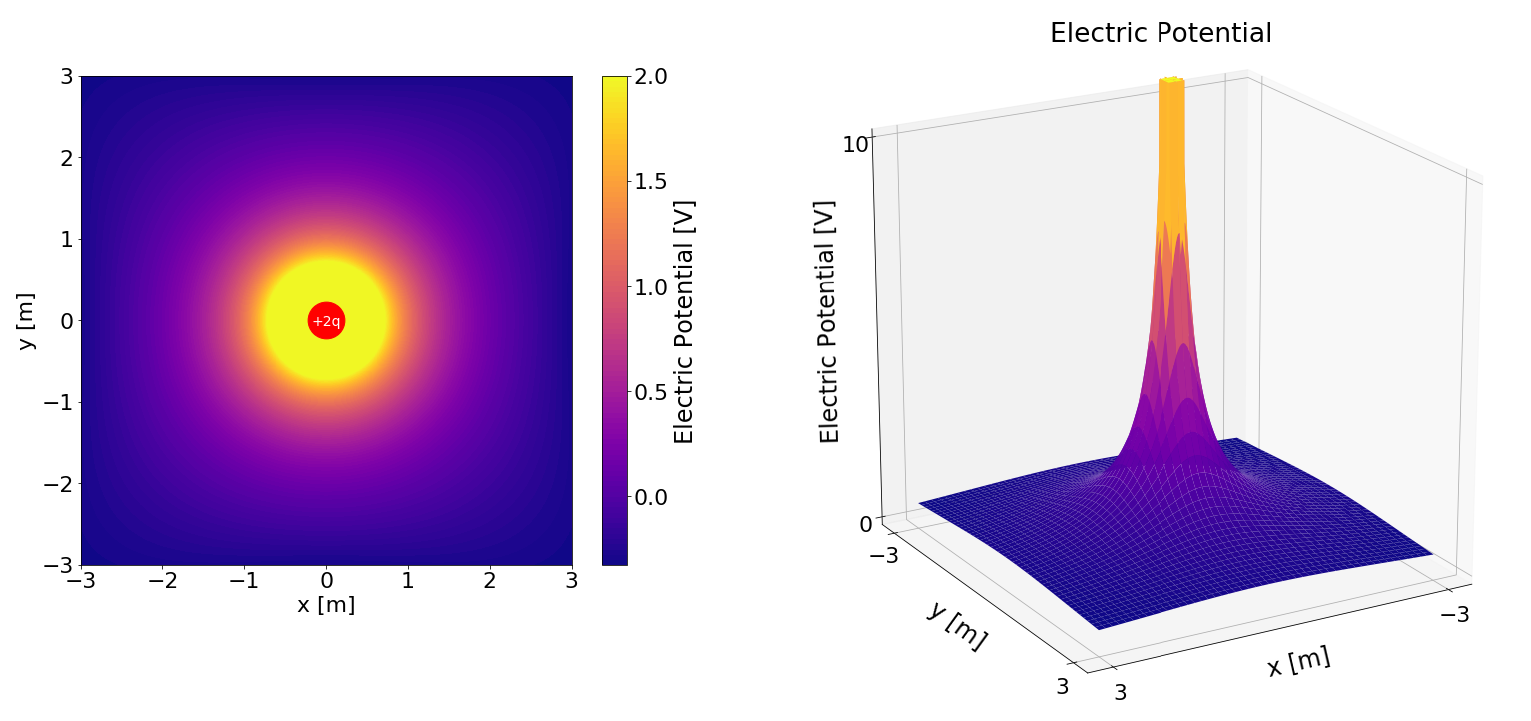
\includegraphics[width=1\linewidth]{files/1pos-10664d2fe2193f689c1cd55a58c46974.png}
\caption[]{Electric potential heat map (left) and surface plot (right) near a single positive charge.}
\label{fig:potential:1pos}
\end{figure}

The most common way to visualize the electric potential is to draw ``contour lines'', similar to how one draws contour lines on a geographical map. On a geographical map, contours correspond to lines of constant altitude, which are also lines of constant gravitational potential energy. Similarly, we can draw lines of constant electric potential. Lines of constant potential are called ``equipotential lines''. In three dimensions, regions of constant electric potential can be surfaces or volumes, called ``equipotential surfaces/volumes''.

The \textbf{electric field vector is always perpendicular to equipotential lines/surfaces}. At any point in space, the electric field vector points opposite to the gradient of the electric potential, since $\vec E= -\nabla V$. This means that the electric field points in the direction where the potential decreases the fastest, which must be perpendicular to the direction where the potential stays the same (i.e. the equipotential lines). Another way to think about this is to consider a charge moving along an equipotential. By definition, the electric potential energy of the charge does not change if its moves along an equipotential. As a result, the electric force/field cannot do any work on the charge, and so must be perpendicular to the path of the charge.

In order to draw equipotential lines, you can start by drawing electric field lines, and then draw (closed) contour lines that are everywhere perpendicular to the electric field lines. This is illustrated in Figure~\ref{fig:potential:2pos1neg}.

\begin{figure}[!htbp]
\centering
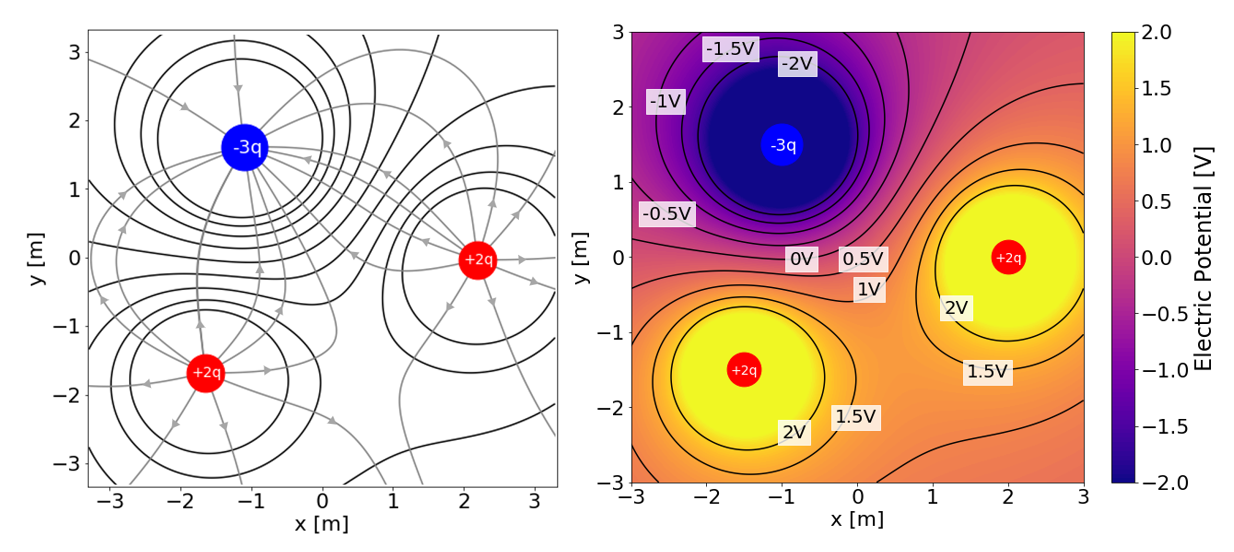
\includegraphics[width=1\linewidth]{files/2pos1neg-e8dd5cf26924b9dc21d27caecd4af793.png}
\caption[]{The electric field and equipotential lines caused by two $+2q$ charges and one $-3q$ charge (left) and its corresponding electric potential heatmap (right).}
\label{fig:potential:2pos1neg}
\end{figure}

In general, it is preferable to draw equipotential lines at equal increments of potential (e.g. every $10 {\rm V}$). For example, the equipotential lines for a point charge located at the origin consist of concentric circles centred at the origin (in three dimensions, this results in concentric spherical equipotential surfaces). If we define $0 {\rm V}$ to be at infinity, the electric potential is given by:
\begin{equation}
V(r)=\frac{kQ}{r}
\end{equation}
In order to draw equipotential lines every $10 {\rm V}$, the radii of the corresponding equipotential circles, for $V=10 {\rm V}$, $V=20 {\rm V}$, $V=30 {\rm V}$, etc., are given by:
\begin{equation}
r&=\frac{kQ}{V}\\
r_{10V}&=\frac{kQ}{(10 {\rm V})}\quad r_{20V}=\frac{kQ}{(20 {\rm V})}\quad r_{30V}=\frac{kQ}{(30 {\rm V})}\quad \dots
\end{equation}

\subsubsection{Calculating electric potential from charge distributions}

In this section, we give two examples of determining the electric potential for different charge distributions. We have two methods that we can use to calculate the electric potential from a distribution of charges:

\begin{enumerate}
\item Model the charge distribution as the sum of infinitesimal point charges, $dq$, and add together the electric potentials, $dV$, from all charges, $dq$. This requires that one choose $0 {\rm V}$ to be located at infinity, so that the $dV$ are all relative to the same point.
\item Calculate the electric field (either as a integral or from Gauss' Law), and use:
\end{enumerate}
\begin{equation}
\Delta V &=V(\vec r_B)-V(\vec r_A)=-\int_A^B  \vec E\cdot d\vec r
\end{equation}
The first method is similar to how we calculated the electric field for distributed charges in Section~\ref{chapter:chargesfields}, but with the simplification that we only need to sum scalars instead of vectors. The second method was already introduced in this chapter.

\begin{framed}
\textbf{Example 17.4}\\
A ring of radius $R$ carries a total charge $+Q$. Determine the electric potential a distance $a$ from the centre of the ring, along the axis of symmetry of the ring. Assume that zero electric potential is defined at infinity.

\begin{framed}
\textbf{Solution}\\
Figure~\ref{fig:potential:ring} shows a diagram of the ring, and our choice of infinitesimal charge, $dq$.

\begin{figure}[!htbp]
\centering
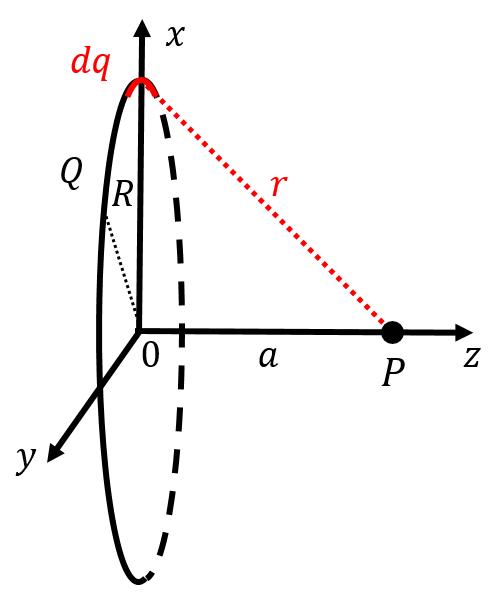
\includegraphics[width=0.3\linewidth]{files/ring-0d66df454bf3b2c8ce93155a3488ea0e.png}
\caption[]{Determining the electric potential on the axis of a ring of radius $R$ carrying charge $Q$.}
\label{fig:potential:ring}
\end{figure}

In order to calculate the electric potential at point, $P$, with $0 {\rm V}$ defined to be at infinity, we first calculate the infinitesimal potential at $P$ from the infinitesimal point charge, $dq$:
\begin{equation}
dV=k\frac{dq}{r}
\end{equation}
The total electric potential is then the sum (integral) of these potentials:
\begin{equation}
V=\int dV=\int k\frac{dq}{r} = \frac{k}{r}\int dq=k\frac{Q}{r}=k\frac{Q}{\sqrt{a^2+R^2}}
\end{equation}
where we recognized that $k$ and $r$ are the same for each $dq$, so that they could factor out of the integral. $\int dq=Q$ is then just the sum of the infinitesimal charges, which must add to the charge of the ring.

\textbf{Discussion:} In this example, we determined the electric potential, relative to infinity, a distance $a$ from the centre of a charge ring, along its axis of symmetry. We modelled the ring as being made of many infinitesimal point charges, and summed together the infinitesimal electric potentials from those charges relative to infinity. This was much simpler than determining the electric field, since electric potential is a scalar and we do not need to consider how the components from different $dq$ along the ring will cancel.
\end{framed}
\end{framed}

\begin{framed}
\textbf{Example 17.5}\\
A long, thin, straight wire carries uniform charge per unit length, $\lambda$. The electric potential difference between points located at distances $r_B=2 {\rm cm}$ and $r_A=1 {\rm cm}$ from the wire is found to be $V(r_B) -V(r_A)= -100 {\rm V}$. What is the linear charge density on wire, $\lambda$?

\begin{figure}[!htbp]
\centering
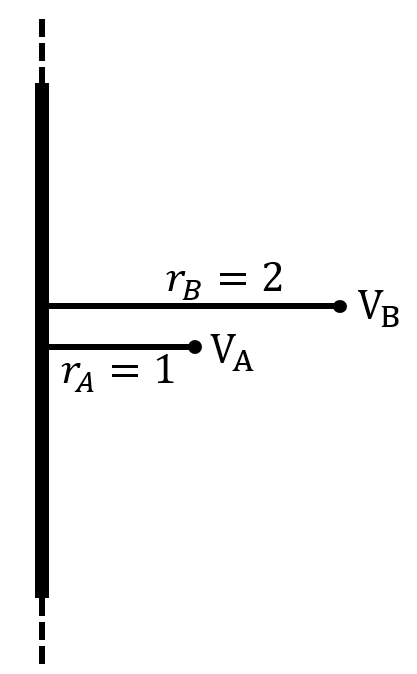
\includegraphics[width=0.2\linewidth]{files/infinitewire-99f6a9acd349bbbe385425382255e9eb.png}
\caption[]{A long thin wire with measurements of electric potential at varying points.}
\label{fig:potential:infinitewire}
\end{figure}

\begin{framed}
\textbf{Solution}\\
In this case, we can use Gauss' Law to determine the electric field at a certain distance from the wire. From that, we can calculate the electric potential difference between any two points near the wire, and thus the charge density on the wire.

By using a cylindrical surface of length, $L$, and radius, $r$, we can use Gauss' Law to determine the field at a distance, $r$, from the wire:
\begin{equation}
\oint \vec E\cdot d\vec A&=\frac{Q^{enc}}{\epsilon_0}\\
2\pi r L E&= \frac{\lambda L}{\epsilon_0}\\
\therefore \vec E(r)&=\frac{\lambda}{2\pi\epsilon_0 r}\hat r
\end{equation}
Using the electric field, we can calculate the potential difference between two points that are at distances, $r_A$ and $r_B$, from the wire:
\begin{equation}
\Delta V &=V(r_B)-V(r_A)\\
&=-\int_{r_A}^{r_B}  \vec E\cdot d\vec r\\
&=-\int_{r_A}^{r_B}  \left( \frac{\lambda}{2\pi\epsilon_0 r}\hat r \right)\cdot d\vec r\\
&=-\frac{\lambda}{2\pi\epsilon_0}\int_{r_A}^{r_B}   \frac{1}{r}\hat r \cdot d\vec r\\
&=-\frac{\lambda}{2\pi\epsilon_0}\int_{r_A}^{r_B}   \frac{1}{r}dr\\
&=-\frac{\lambda}{2\pi\epsilon_0}\left[|\ln(r)|\right]_{r_A}^{r_B} \\
&= -\frac{\lambda}{2\pi\epsilon_0}\ln\left(\frac{r_B}{r_A}\right)\\
\therefore\Delta V &=\frac{\lambda}{2\pi\epsilon_0}\ln\left(\frac{r_A}{r_B}\right)
\end{equation}
where, in the second last line, we removed the absolute value from the logarithm, since $r_A<r_B$, and in the last line, we removed the minus sign by inverting the argument of the logarithm. Since we know the potential difference, $\Delta V$, for two points located at distances $r_B=2 {\rm cm}$ and $r_A=1 {\rm cm}$, we can determine the charge density on the wire:
\begin{equation}
\Delta V &=V(r_B)-V(r_A)=-100 {\rm V}\\
\Delta V &=\frac{\lambda}{2\pi\epsilon_0}\ln\left(\frac{r_A}{r_B}\right)\\
\therefore \lambda &= \frac{2\pi\epsilon_0\Delta V}{\ln\left(\frac{r_A}{r_B}\right)}\\
&=\frac{2\pi(8.85\times 10^{-12} {\rm C^2\cdot N^{-1}\cdot m^{-2}})(-100 {\rm V})}{\ln\left(\frac{1}{2}\right)}\\
&=8.02\times 10^{-9} {\rm C/m}
\end{equation}
where, again, one needs to be very careful with the signs! Note that it also makes sense that the potential difference, $\Delta V =V(r_B) -V(r_A)$, is negative, since $r_A$ is closer to the positively charged wire. A positive charge at rest would move away from the positively charged wire, from $r_A$ to $r_B$, from high potential to low potential.

\textbf{Discussion:} In this example, we showed how to determine the electric potential near an infinitely long charged wire by using the electric field that we determined from Gauss' Law. By knowing the potential difference between two points near the wire, we were then able to infer the charge density on the wire.
\end{framed}
\end{framed}

\subsubsection{Electric field and potential at the surface of a conductor}

Conducting materials are always equipotential surfaces (or volumes) if charges are not moving inside the conductor. This is because the electric field inside a conductor is always zero and thus, a charge moving through a conductor experiences no electric force and its electrical potential energy will be constant. Similarly, because the electric field must always be perpendicular to an equipotential, electric field lines are always perpendicular to the surface of a conductor (in electrostatics).

If we consider a conducting sphere of radius $R$ and charge $+Q$, the electric field at the surface of the sphere is given by:
\begin{equation}
E=k\frac{Q}{R^2}
\end{equation}
as we found in Section~\ref{chapter:gauss}. If we define electric potential to be zero at infinity, then the electric potential at the surface of the sphere is given by:
\begin{equation}
V=k\frac{Q}{R}
\end{equation}
In particular, the electric field at the surface of the sphere is related to the electric potential at its surface by:
\begin{equation}
E=\frac{V}{R}
\end{equation}
Thus, if two spheres are at the same electric potential, the one with the smaller radius will have a stronger electric field at its surface.

Because a conducting sphere is symmetric, the charges will distribute themselves symmetrically around the whole outer surface of the sphere. The charge per unit area, $\sigma$, at the surface of the sphere is thus given by:
\begin{equation}
\sigma &= \frac{Q}{4\pi R^2}
\end{equation}
The charge density can be related to the electric field at the surface of the sphere:
\begin{equation}
E&=k\frac{Q}{R^2}=k\frac{4\pi R^2\sigma}{R^2}=4\pi\sigma k=\frac{\sigma}{\epsilon_0}
\end{equation}
where in the last equality, we used $k$ with $\epsilon_0$ and confirmed the general result from Section~\ref{sec:gauss:conductors}, where we determined the electric field near a conductor with surface charge $\sigma$.

Consider a sphere of radius $R_1$ that carries total charge, $+Q$. A neutral second, smaller, conducting sphere, of radius $R_2$, is then connected to the first sphere, using a conducting wire, as in Figure~\ref{fig:potential:twospheres}.

\begin{figure}[!htbp]
\centering
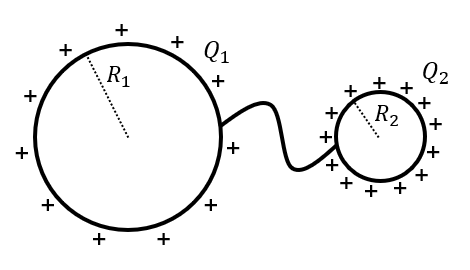
\includegraphics[width=0.5\linewidth]{files/twospheres-db4e08e96dc924ae5b6fd51098023f44.png}
\caption[]{Two conducting spheres are connected by a conducting wire. The charge $Q$ that was originally on the larger sphere distributes itself onto the two spheres.}
\label{fig:potential:twospheres}
\end{figure}

Because the charges on the large sphere can move around freely, some of them will move to the smaller sphere. Very quickly, the charges will stop moving and the spheres of radius $R_1$ and $R_2$ will end up carrying charges $Q_1$ and $Q_2$, respectively (we assume that the wire is small enough that negligible amounts of charge are distributed on the wire). Since the two conducting spheres are connected by a conductor, they form an equipotential, and are thus at the same voltage, $V$, relative to infinity. Since the two spheres are at the same electric potential, the electric field at the surface of each sphere are related:
\begin{equation}
E_1&=\frac{V}{R_1}\\
E_2&=\frac{V}{R_2}\\
\therefore \frac{E_2}{E_1}&=\frac{R_1}{R_2}\\
\therefore E_2&=E_1\frac{R_1}{R_2}
\end{equation}
and the electric field at the surface of the smaller sphere, $E_2$, is stronger since $R_2<R_1$. We can also compare the surface charge densities on the two spheres:
\begin{equation}
E_1&=\frac{\sigma_1}{\epsilon_0}\\
E_2&=\frac{\sigma_2}{\epsilon_0}\\
\therefore \frac{\sigma_2}{\sigma_1}&=\frac{E_2}{E_1}=\frac{R_1}{R_2}\\
\therefore \sigma_2&=\sigma_1 \frac{R_1}{R_2}
\end{equation}
and we find that the charge density is higher on the smaller sphere. Thus, there are more charges per unit area on the smaller sphere than the bigger sphere.

We can generalize this model to describe charges on any charged conducting object. If charges are deposited on a conducting object that is not a sphere, as in Figure~\ref{fig:potential:chargeblob}, they will not distribute themselves uniformly. Instead, there will be a higher charge density (charges per unit area), near parts of the object that have a small radius of curvature, just as the charge density was higher on the smaller sphere described above. As a consequence of the higher concentration of charges near the ``pointier'' parts of the object, the electric field at the surface will be the strongest in those regions.

\begin{figure}[!htbp]
\centering
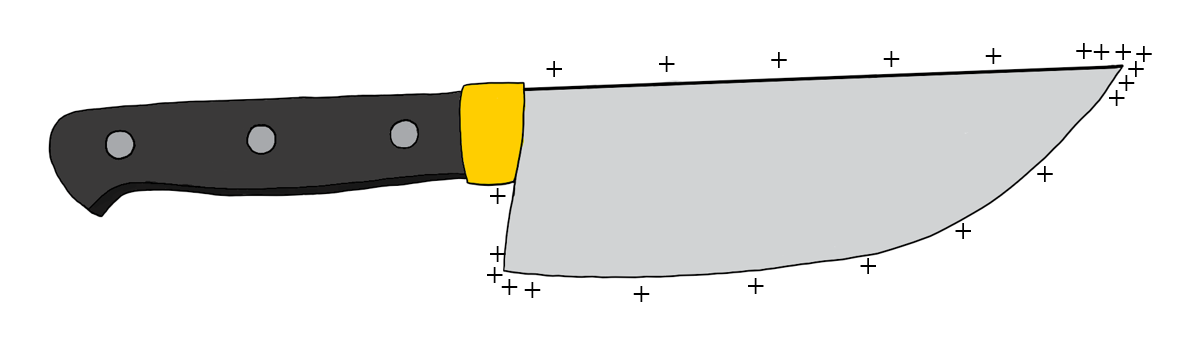
\includegraphics[width=0.65\linewidth]{files/chargeblob-18e4c296aa731c7a6315c4332e948ff6.png}
\caption[]{On an uneven conductor, charges will accumulate on the sharper points, where the radius of curvature is the smallest.}
\label{fig:potential:chargeblob}
\end{figure}

In air, if the electric field exceeds a magnitude of approximately $3\times 10^{6} {\rm V/m}$, the air is said to ``electrically break down''. The strong electric field can remove electrons from atoms in the air, ionizing the air in a chain reaction and making it conductive. Thus, if the electric field at a point on the surface of a conductor is very strong, the air near that point will break down, and charges will leave the conductor, through the air, to find a location with lower electric potential energy (usually the ground). Electric breakdown is what we experience as a spark (or lightning, on a larger scale), and is usually a discrete (and potentially dramatic) event. Corona discharge is another mechanism whereby the strong electric field can make the air conductive, but in this case, charges leak into the air more gradually, unlike in the case of electrical break down. Charges leaking into air through Corona discharge will emit a faint blueish light (the ``Corona'') as well as an audible hissing sound.

Objects that are designed to hold a high electric potential (for example the electrodes on high voltage lines) are usually made very carefully so that they have a very smooth surface and no sharp edges. This reduces the risk of breakdown or Corona discharge at the surface which would result in a loss of charge.

Contrary to popular belief, lightning rods are not designed to attract lightening. Instead, lightning rods are designed to be conductors with a very sharp point, so that Corona discharge can occur at their tip. This allows charges to slowly leak off from the Earth into the cloud through Corona discharge, thereby reducing the potential difference between the cloud and Earth so that a lightning strike (electrical breakdown) does not occur. When a lightning strike does occur, it will hit the lightning rod, since the electric field at the top of the rod is high and that is the most likely point for the air to break down; but, that is not the goal of the lightning rod!

\subsubsection{Capacitors}\label{sec:potential:capacitors}

Capacitors are common electronic devices that are used to store electric charge for a variety of applications. A capacitor is usually constructed with two conducting plates (called ``terminals'' or ``electrodes'') separated by either air or an insulating material.

\begin{figure}[!htbp]
\centering
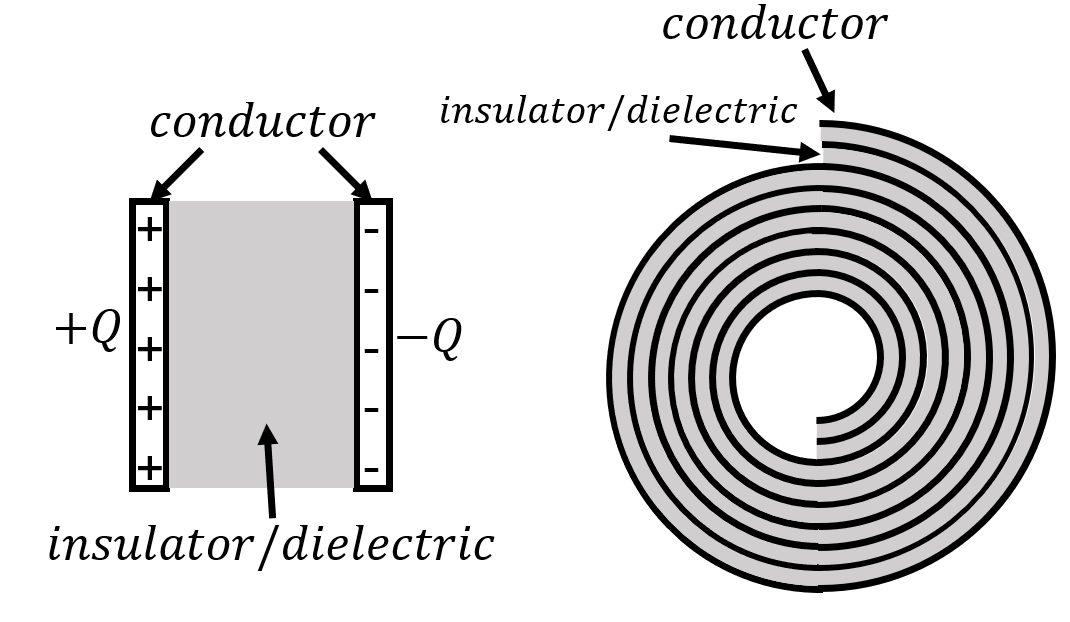
\includegraphics[width=0.5\linewidth]{files/capacitors-c81e377aa34e65c60dc580ecd7789fe2.png}
\caption[]{Two examples of capacitors. The left panel shows a ``parallel plate'' capacitor, and the right panel shows a cylindrically shaped capacitor obtained by ``rolling up'' a parallel plate capacitor.}
\label{fig:potential:capacitors}
\end{figure}

Figure~\ref{fig:potential:capacitors} shows two examples of capacitors. The left panel shows a ``parallel plate'' capacitor, consisting of two conducting plates separated by air or an insulator. The plates are conducting in order for one to be able to easily add and remove charge to the plates. The plates always hold equal and opposite charges. The right panel shows a more practical implementation of a capacitor that could be used in a circuit, which is simply made by ``rolling up'' a parallel plate capacitor (with an insulator instead of air separating the plates so that they do not touch).

\paragraph{Capacitance}

As long as the quantities of charge involved are not too large, it has been observed that the amount of charge, $Q$, that can be stored on a capacitor\footnote{This is the amount of charge on one of the plates. As a whole, the capacitor is neutral.}, is linearly proportional to the potential difference, $\Delta V$, between the two plates:
\begin{equation}
Q\propto \Delta V
\end{equation}
\begin{equation}
\boxed{Q=C\Delta V}
\end{equation}
The constant of proportionality, $C$, between charge and potential difference across the capacitor (usually called voltage across the capacitor) is called ``capacitance'', and has S.I. units of ``Farads'' (${\rm F}$). The capacitance of a particular capacitor is a measure of how much charge it can hold at given voltage and depends on the geometry of the capacitor as well as the material between the terminals. If too much charge is placed on a capacitor, the material between the two plates will break down, and a spark will usually damage the capacitor as well as discharge it.

We can easily calculate the capacitance of a parallel plate capacitor. We model the capacitor as being made of two conducting plates, each with area, $A$, separated by a distance, $L$, and holding charge with magnitude, $Q$. The surface charge density on one of the plates, $\sigma$, is just given by:
\begin{equation}
\sigma =\frac{Q}{A}
\end{equation}
In Example~17.3, we found an expression for the potential difference between two parallel plates:
\begin{equation}
\Delta V &= \frac{\sigma}{\epsilon_0}L=\left(\frac{L}{A\epsilon_0}\right)Q
\end{equation}
Comparing with, $Q=C\Delta V$, the capacitance of the parallel plate capacitor is found to be:
\begin{equation}
C=\epsilon_0\frac{A}{L}
\end{equation}
It makes sense that the capacitance, the amount of charge that can be stored at a given voltage, increases if the plates have a larger area (more space for charges), and decreases if the plates are further apart . \%todo: ask (smaller electric field).

Capacitors are used in many touch screens. For example, these might be made of glass (an insulator), with a thin metal coating that one touches to interact with the screen (one of the plates). As you touch the metal plate, you effectively change the capacitance of the screen, which can be sensed and modelled to determine the location of your finger(s). Modern touch screens have many capacitors built directly into the screen, and function based on this principle.

\begin{framed}
\textbf{Checkpoint}\\
A capacitor holds $0.2 {\rm C}$ of charge when it has a potential difference of $500 {\rm V}$ between its plates. If the same capacitor holds $0.15 {\rm C}$ of charge,  what is the potential difference between its plates?

\begin{enumerate}
\item $375 {\rm V}$.
\item $500 {\rm V}$.
\item $75 {\rm V}$.
\item $150 {\rm V}$.
\end{enumerate}

\begin{framed}
\textbf{Answer}\\
\begin{enumerate}
\item
\end{enumerate}
\end{framed}
\end{framed}

\paragraph{Dielectric materials}

In practice, capacitors always have an insulating material between the two plates. The material is chosen to have a higher breakdown voltage than air, so that more charges can be stored before a breakdown occurs. It has also been experimentally observed that the capacitance increases with certain materials, so called ``dielectric materials''. A dielectric material has a ``dielectric constant'', $K$, defined to be the amount by which the capacitance increases:
\begin{equation}
C=KC_0
\end{equation}
where $C$ is the capacitance with the material in place, and $C_0$ is the capacitance when there is a vacuum between the plates (the dielectric constant of air is very close to 1). Often, rather than the dielectric constant, one uses the ``permittivity'', $\epsilon$, of a material:
\begin{equation}
\epsilon=K\epsilon_0
\end{equation}
based on the permittivity of free space, $\epsilon_0$. The capacitance of a parallel plate capacitor, with a material that has permittivity, $\epsilon$, is thus given by:
\begin{equation}
C=K\epsilon_0\frac{A}{L}=\epsilon\frac{A}{L}
\end{equation}
Dielectric materials are made of molecules that can be polarized (such as water), namely molecules that have a non-zero electric dipole moment. When the dielectric material is placed between the plates, the dipoles inside the material align themselves with the electric field from the plates. This leads to a second electric field, from the dipoles, in the opposite direction of the field from the plates, thus reducing the total electric field between the plates. This, in turn, allows more charges to be held on the plate for a given voltage. This is illustrated in Figure~\ref{fig:potential:polarizeddipoles}

\begin{figure}[!htbp]
\centering
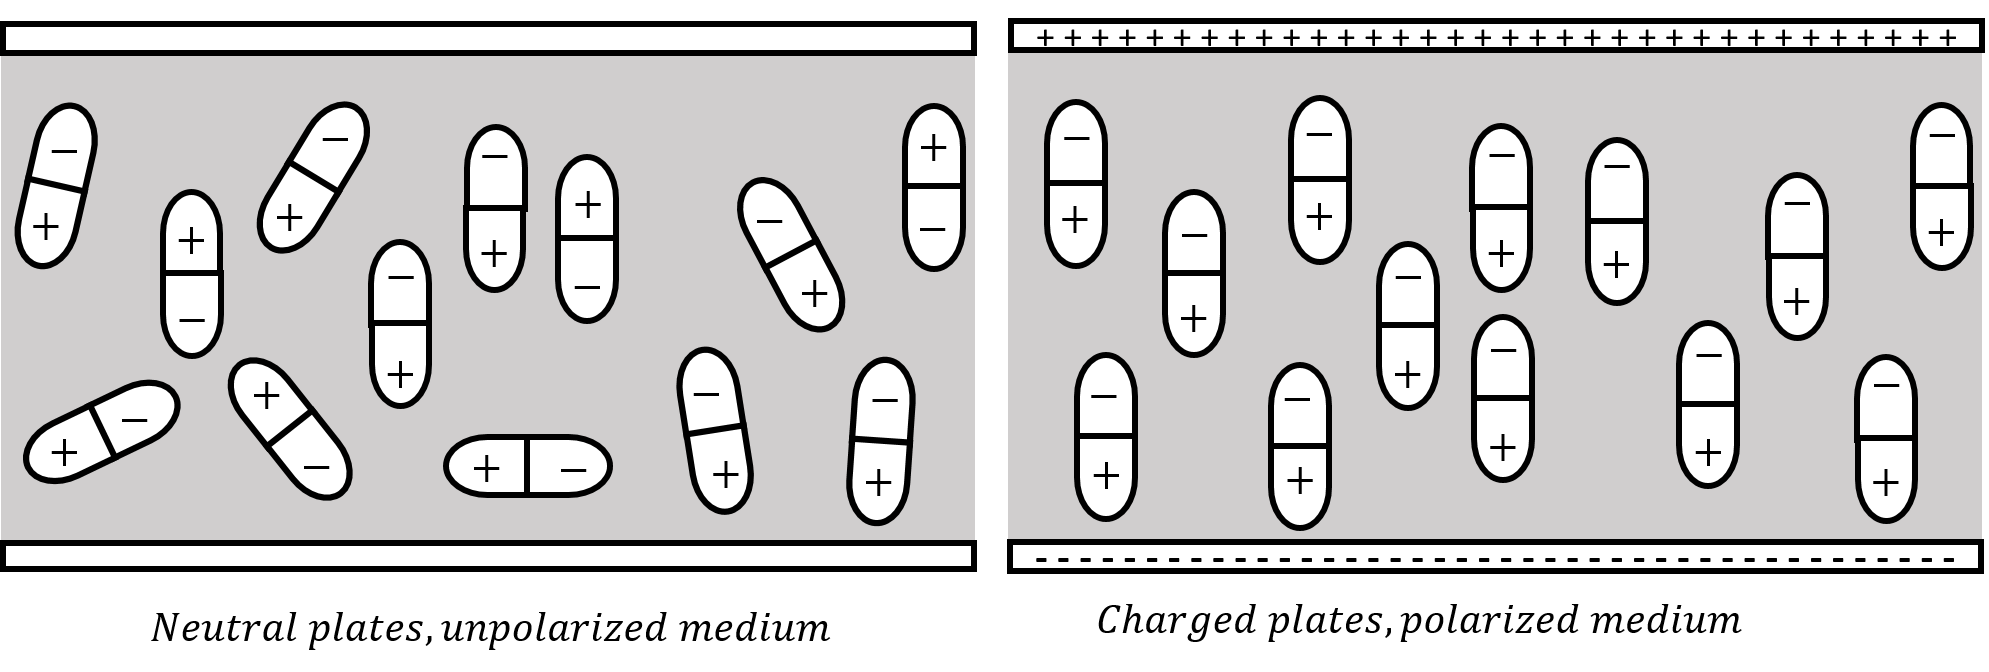
\includegraphics[width=0.8\linewidth]{files/polarizeddipoles-e5ce4de56894724c087e06f93a23086e.png}
\caption[]{A dielectric material is placed between the two plates of a capacitor. The electric dipoles in the dielectric have random orientations when the plates are neutral (left panel). When the plates are charged (right panel), the dipoles align themselves with the field from the plates, allowing more charge to be on the plates at a given potential difference.}
\label{fig:potential:polarizeddipoles}
\end{figure}

Note that, in a dielectric material with permittivity $\epsilon$, Gauss's Law is modified to read:
\begin{equation}
\oint \vec E\cdot d\vec A=\frac{Q^{enc}}{\epsilon}
\end{equation}
where the permittivity of free space, $\epsilon_0$, is simply replaced with the permittivity of the material, $\epsilon$.

\paragraph{Energy stored in a capacitor}

The charges stored on a capacitor have electric potential energy: if one were to place a conductor between the plates, charges would immediately conduct from one plate to the other and gain kinetic energy. We can model the amount of energy stored on the capacitor by considering how much work it takes to place the charges on the capacitor.

Imagine that both plates on the capacitor start with a charge of magnitude $q$. We then remove an infinitesimal negative charge, with magnitude $dq$, from the positive plate and place it on the negative plate. This required work, since we had to pull this negative charge away from the positive plate. If the potential difference across the plates is $\Delta V$, then we had to do an amount of work given by:
\begin{equation}
dW = \Delta Vdq
\end{equation}
since the charge $dq$ has now gained potential energy, $\Delta Vdq$. The potential difference is dependent on the (constant) capacitance of the capacitor, and the amount of charge, $q$, already stored on the plates:
\begin{equation}
q &= C\Delta V\\
\therefore \Delta V&=\frac{q}{C}
\end{equation}
In order to determine the work required to transfer a total amount of charge, $Q$, we sum the work in transferring each infinitesimal charge, $dq$:
\begin{equation}
W=\int dW=\int_0^Q \Delta Vdq=\int_0^Q \frac{q}{C}dq=\frac{1}{2}\frac{Q^2}{C}
\end{equation}
Thus, the total potential energy that is stored on a capacitor is given by:
\begin{equation}
U = \frac{1}{2}\frac{Q^2}{C} = \frac{1}{2}C(\Delta V)^2=\frac{1}{2}Q\Delta V
\end{equation}
where we made use of $Q=C\Delta V$ to show the formula with different choices of variables. In either case, the amount of energy that is stored increases with the amount of charge, the capacitance, and the voltage across the capacitor. Capacitors are useful because this energy can be released quickly, as in the bright flash of light required for flash photography.

\subsubsection{Summary}

The electric force is conservative, so we can define a potential energy function, $U(\vec r)$. The potential energy function for a point charge, $q$, at position $\vec r$, relative to a point charge, $Q$, is given by:
\begin{equation}
U(\vec r) = \frac{kQ}{r}q + C
\end{equation}
where $C$ is an arbitrary constant, since only differences in potential energy are physically meaningful (as they correspond to work). Note that the sign of the electrical potential energy will depend on the relative sign of $q$ and $Q$. If a collection of charges are held together, the total electrical potential energy that is stored is called ``electrostatic potential energy''.

Similarly to how the electric field, $\vec E(\vec r)$, corresponds to electric force per unit charge, ``electric potential'', $V(\vec r)$, corresponds to electric potential energy per unit charge. The electric potential at a position, $\vec r$, relative to a point charge, $Q$, is given by:
\begin{equation}
V(\vec r) =\frac{U(\vec r)}{q}= \frac{kQ}{r} + C'
\end{equation}
and also depends on an arbitrary constant, $C'$, since only differences in electric potential will lead to differences in potential energy. The value of the electric potential, $V$, at some position in space, $\vec r$, allows us to determine the electric potential energy, $U$, at that position for any charge, $q$:
\begin{equation}
U = qV
\end{equation}
This is analogous to determining the force on a charge, $q$, when we know the electric field at some point in space:
\begin{equation}
\vec F = q \vec E
\end{equation}
Differences in electric potential are called ``voltages'', and the S.I. unit of potential is called the ``volt'' (V). In S.I. units, the electric field is often expressed in units of volts per metre (V/m).

When a particle with charge $q$ changes position such that the corresponding change in electric potential is $\Delta V$, the particle's potential energy will change by:
\begin{equation}
\Delta U = q\Delta V
\end{equation}
In particular, a negative charge will experience a decrease in potential energy when the electric potential increases, whereas a positive charge will experience an increase in potential energy when the electric potential increases. This reflects the fact that the electric force associated with the electric potential will act in opposite directions on a positive and a negative charge.

In order to describe the energies of particles interacting with electric forces, it is more convenient to use the ``electron volt'' instead of the Joule. An electron volt is defined as the energy that is gained by a charge with a magnitude $e$ (the magnitude of the charge of the electron) when accelerated through a potential difference of $\Delta V=1 {\rm V}$:
\begin{equation}
1 {\rm eV}&=(e)(1 {\rm V})=1.6\times 10^{-19} {\rm J}
\end{equation}

The electric potential function can be determined in two different ways:

\begin{enumerate}
\item By modelling the charge distribution as the sum of infinitesimal point charges, $dq$, and adding together the electric potentials, $dV$, from all charges, $dq$. This requires that one choose $0 {\rm V}$ to be located at infinity, so that the $dV$ are all relative to the same point.
\item By calculating the electric field (either as a integral or from Gauss' Law), and using:
\end{enumerate}
\begin{equation}
\Delta V &=V(\vec r_B)-V(\vec r_A)=-\int_A^B  \vec E\cdot d\vec r
\end{equation}
It is worth noting that one needs to be very careful with the signs when using the above integral. In particular note that one takes the negative of the integral, from $A$ to $B$, to determine the potential at $B$ minus the potential at $A$.

Similarly, one can determine the value of the electric field, $\vec E(\vec r)=\vec E(x,y,z)$, from the electric potential, $V(\vec r)=V(x,y,z)$:
\begin{equation}
\vec E(x,y,z) = -\nabla V =-\frac{\partial V}{\partial x}\hat x-\frac{\partial V}{\partial y}\hat y-\frac{\partial V}{\partial z}\hat z
\end{equation}
where, $\nabla V$, is the gradient of the electric potential.

The electric potential can be visualized in a number of ways. The most common is to draw contours of constant electric potential, akin to the contours on geographical maps that are used to show regions of constant altitude (i.e. constant gravitational potential energy).

Regions of constant electric potential are called ``equipotentials'', and can be lines, surfaces or volumes. Equipotentials are always perpendicular to the electric field. In electrostatics (when charges are not moving), the electric field in a conductor must be zero, so that a conductor always forms an equipotential, and the electric field at the surface of a conductor is always perpendicular to the surface.

When charges are placed on a conductor, they will spread out along the outer surface of the conductor. The surface density of charges will be the highest where the conductor has the smallest radius of curvature (e.g. at a sharp point). Consequently, the electric field at the surface of a charged conductor is highest near sharp points.

Capacitors are devices that are used to store charge. They are usually made using two conducting plates (``terminals'' or ``electrodes'') that hold equal and opposite charge, $Q$, at a fixed potential difference, $\Delta V$ , between the electrodes. The amount of charge that is stored on the capacitor is observed to be proportional to the potential difference between the electrodes:
\begin{equation}
Q=C\Delta V
\end{equation}
where the constant of proportionality, $C$, is called the ``capacitance'' of the capacitor. The S.I. unit of capacitance is the ``Farad'' (F). The capacitance of a capacitor depends on its geometry (e.g. its size) and the materials that it is placed between the electrodes.

Usually, one places a dielectric material between the two electrodes in order to increase the capacitance, and to reduce the risk of breakdown. If that material has a ``dielectric constant'', $K$, then the capacitance is given by:
\begin{equation}
C=KC_0
\end{equation}
where, $C_0$, corresponds to the capacitance if there were vacuum between the electrodes. The dielectric constant of air is very close to 1, so that a capacitor in air is very similar to a capacitor in vacuum. A dielectric material is one that is made of molecules that can be polarized under the presence of an electric field; that is, the molecules have an electric dipole moment. When the molecules in a material are polarized, this reduces the total electric field in the material, which increases the capacitance of the capacitor. Inside a dielectric material, we can define the ``permittivity'', $\epsilon$, as:
\begin{equation}
\epsilon=K\epsilon_0
\end{equation}
where $\epsilon_0$ is the permittivity of free space. Within a dielectric material, Gauss' Law is modified to:
\begin{equation}
\oint \vec E \cdot d\vec A=\frac{Q^{enc}}{\epsilon}
\end{equation}

Since charges are held at a fixed potential difference on a capacitor, capacitors are a way of storing electric potential energy. The amount of electric potential energy stored in a capacitor with capacitance, $C$, when the capacitor has a potential difference, $\Delta V$, across its electrodes, is given by:
\begin{equation}
U = \frac{1}{2}\frac{Q^2}{C} = \frac{1}{2}C(\Delta V)^2=\frac{1}{2}Q\Delta V
\end{equation}

\begin{framed}
\textbf{Important Equations}\\
\textbf{Electric potential energy from a point charge}
\begin{equation}
U(r)=\frac{kQq}{r}+C
\end{equation}

\textbf{Electric potential}
\begin{equation}
V=\frac{U}{q}
\end{equation}

\textbf{Electric potential:}
\begin{equation}
\Delta V = V(\vec r_B)-V(\vec r_A)\\
\Delta V = -\int_{A}^{B}\vec E \cdot d\vec r
\end{equation}

\textbf{Electric field:}
\begin{equation}
\vec E=-\nabla V =-\frac{\partial V}{\partial x}\hat x-\frac{\partial V}{\partial y}\hat y-\frac{\partial V}{\partial z}\hat z
\end{equation}

\textbf{Electric potential from a point charge}
\begin{equation}
V(r)=\frac{kQ}{r}+C
\end{equation}

\textbf{Electric potential between two parallel plates}
\begin{equation}
\Delta V = EL
\end{equation}

\textbf{Charge stored in a capacitor:}
\begin{equation}
Q = C\Delta V
\end{equation}

\textbf{Energy stored in a capacitor}
\begin{equation}
U = \frac{1}{2}\frac{Q^2}{C} = \frac{1}{2}C(\Delta V)^2=\frac{1}{2}Q\Delta V
\end{equation}
\end{framed}

\begin{framed}
\textbf{Important Definitions}\\
\begin{itemize}
\item \textbf{Capacitance:} How much charge a capacitor can hold given the potential difference between the terminals of the capacitor. SI units: ${\rm \left[{F}\right]}$. Common variable(s): $C$.
\item \textbf{Dielectric constant:} A constant which is defined as the (dimensionless) ratio of the dielectric permittivity of a substance and the dielectric permittivity of a vacuum. Common variable(s): $K$.
\end{itemize}
\end{framed}

\subsubsection{Thinking about the material}

\begin{framed}
\textbf{Reflect and research}\\
\begin{itemize}
\item Explain how the capacitance can increase when a dielectric material is used.
\item Explain how a corona ring works.
\item Which shapes of electrodes are most common? Why?
\end{itemize}
\end{framed}

\begin{framed}
\textbf{To try at home}\\
\begin{itemize}
\item Try to release a static discharge from your finger to some metal object. Measure the distance between your finger and the metal object at the time of the discharge. Knowing the breakdown voltage of air, what was the potential difference between your finger and the metal object just before the discharge?
\end{itemize}
\end{framed}

\begin{framed}
\textbf{To try in the lab}\\
\begin{itemize}
\item Propose an experiment to measure the point at which various substances experience electric breakdown.
\item Propose an experiment to measure the vacuum permittivity constant ($\epsilon_0$).)
\end{itemize}
\end{framed}

\subsubsection{Sample problems and solutions}

\paragraph{Problems}

\begin{framed}
\textbf{Problem 17.1}\\
A long cylinder of radius $R$ carries a uniform charge per unit volume density, $\rho$. The electric potential at the surface of the cylinder is $V_S = 100 {\rm V}$, where we have chosen $V=0$ at infinity. What is the electric potential inside and outside of the cylinder as a function of $r$, the distance from the centre of the cylinder?
\end{framed}

\begin{framed}
\textbf{Problem 17.2}\\
A capacitor is constructed by placing a concentric conducting cylindrical shell of negligible thickness and inner radius, $R_B$, around a solid conducting cylinder of radius, $R_A$, as illustrated in Figure~\ref{fig:potential:nestedcylinders}. What is the capacitance of this capacitor, where the solid cylinder and the cylindrical shell form the two electrodes?

\begin{figure}[!htbp]
\centering
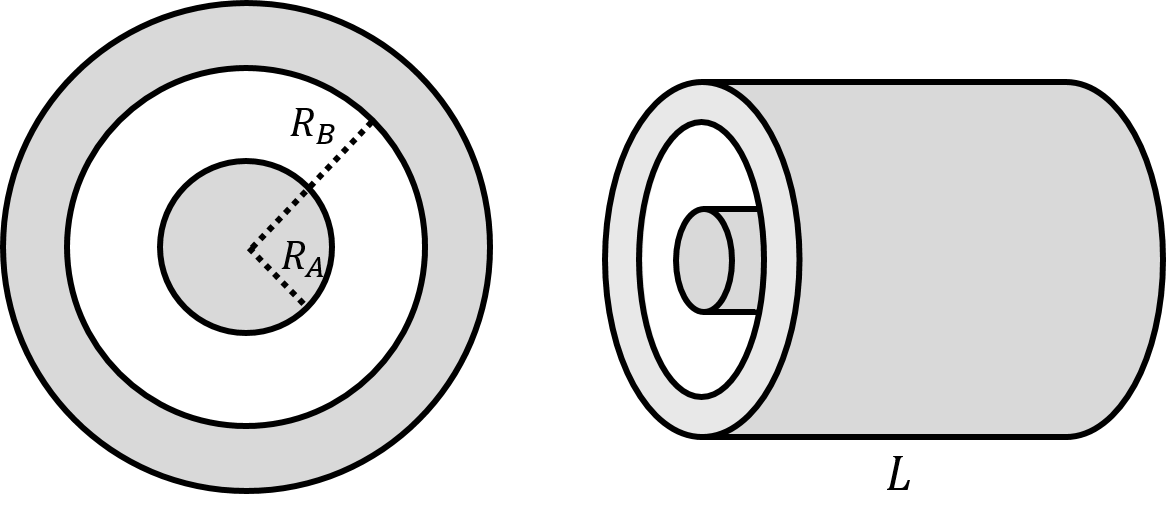
\includegraphics[width=0.7\linewidth]{files/nestedcylinders-72db3afa04c1cef3c4b24e2223231d7f.png}
\caption[]{A capacitor constructed from concentric cylinders.}
\label{fig:potential:nestedcylinders}
\end{figure}
\end{framed}

\paragraph{Solutions}

\begin{framed}
\textbf{Solution 17.1}\\
To determine the electric potential inside and outside of the cylinder, we can use the electric field, which we must first determine. We will do this using Gauss' Law. We will use a Gaussian surface that is a cylinder of radius, $r$, and length, $L$. In both regions, the flux of the electric field will be given by:
\begin{equation}
\int E\cdot dA  = E 2\pi rL
\end{equation}
since the electric field points in the radial direction, away from the centre of the cylinder. Outside of the cylinder ($r>R$), the total charge enclosed is the total charge on a length, $L$, of the cylinder, which has a volume, $\pi R^2 L$:
\begin{equation}
Q^{enc}=\rho \pi R^2 L
\end{equation}
Thus, applying Gauss' Law outside the cylinder, gives the electric field for $r>R$:
\begin{equation}
\int E\cdot dA &= \frac{Q_{enc}}{\epsilon_0}\\
E 2\pi rL &= \frac{\rho \pi R^2 L}{\epsilon_0}\\
\therefore E(r) &= \frac{\rho R^2}{2\epsilon_0r}\quad(r\geq R)
\end{equation}
Inside the cylinder, the enclosed charge is that enclosed by a cylinder of radius, $r$, and length, $L$:
\begin{equation}
Q^{enc}=\rho \pi r^2 L
\end{equation}
Applying Gauss' Law, the electric field inside the cylinder is given by:
\begin{equation}
\int E\cdot dA &= \frac{Q_{enc}}{\epsilon_0}\\
E 2\pi rL &= \frac{\rho \pi r^2 L}{\epsilon_0}\\
\therefore E(r) &= \frac{\rho r}{2\epsilon_0}\quad(r<R)
\end{equation}
Now that we have found the electric field, we can determine the electric potential. What we really want to find is the change in potential when moving a positive point charge from infinity (our 0 \{{\textbackslash}rm V\} point) to the point of interest. We know that the potential at the surface (meaning the potential difference between infinity and the surface) is $V_S=100 {\rm V}$. To find the potential at any point, all we have to do is calculate the potential difference between the surface and the point of interest, and add that to $V_S$.

We will start with the potential inside the cylinder, $r<R$:
\begin{equation}
\Delta V_{r<R} &= V(r)-V_S = -\int_{R}^{r} \vec E\cdot d \vec r\\
&= -\int_{R}^{r} \frac{\rho r}{2\epsilon_0} \hat r \cdot d \vec r\\
&= -\int_{R}^{r} \frac{\rho r}{2\epsilon_0} dr\\
&= -\frac{\rho (r^2-R^2)}{4\epsilon_0}\\
&= \frac{\rho (R^2-r^2)}{4\epsilon_0}\\
\therefore V(r) &= V_S + \frac{\rho (R^2-r^2)}{4\epsilon_0}\\
&=100 {\rm V}+\frac{\rho (R^2-r^2)}{4\epsilon_0}
\end{equation}
Thus, everywhere inside the cylinder, the electric potential is larger than $100 {\rm V}$, since $R^2 -r^2>0$.

We proceed in the same way to determine the potential at position $r$ outside the cylinder, $r>R$:
\begin{equation}
\Delta V_{r>R} &=  V(r) - V_S = -\int_{R}^{r} \vec E\cdot d \vec r\\
&= -\int_{R}^{r} \frac{\rho R^2}{2\epsilon_0r} \hat r \cdot d \vec r\\
&= - \frac{\rho R^2}{2\epsilon_0} \int_{R}^{r} \frac{1}{r}dr\\
&=- \frac{\rho R^2}{2\epsilon_0}(\ln r-\ln R)\\
&=- \frac{\rho R^2}{2\epsilon_0}\ln\left( \frac{r}{R} \right)\\
\therefore V(r) &= V_S - \frac{\rho R^2}{2\epsilon_0} \ln \left( \frac{r}{R} \right)\\
&= 100 {\rm V} - \frac{\rho R^2}{2\epsilon_0} \ln \left( \frac{r}{R} \right)
\end{equation}
Since $r>R$, $\ln (r/R)$ is positive, so the electric potential decreases from as you move away from the cylinder, as expected.
\end{framed}

\begin{framed}
\textbf{Solution 17.2}\\
We will determine the capacitance by relating the potential difference between the electrodes to the charge stored on the electrodes. Using Gauss's Law, we can determine the electric field between the electrodes based on the charge on those electrodes, and from there, we can determine the potential difference. We will ignore the fact that the cylinder has a finite length and that Gauss's Law will not hold near the edges of the cylinder, where the electric field is no longer exactly in the radial direction.

We assume that each electrode carries an equal and opposite charge per unit length, $\lambda$. In order to determine the electric field in the region $R_A<r<R_B$, we consider a cylindrical Gaussian surface of radius $r$ and length $L$, as illustrated in Figure~\ref{fig:potential:nestedcylinderssolution}. The surface encloses a charge $Q^{enc}=\lambda L$ from the inner cylinder.

\begin{figure}[!htbp]
\centering
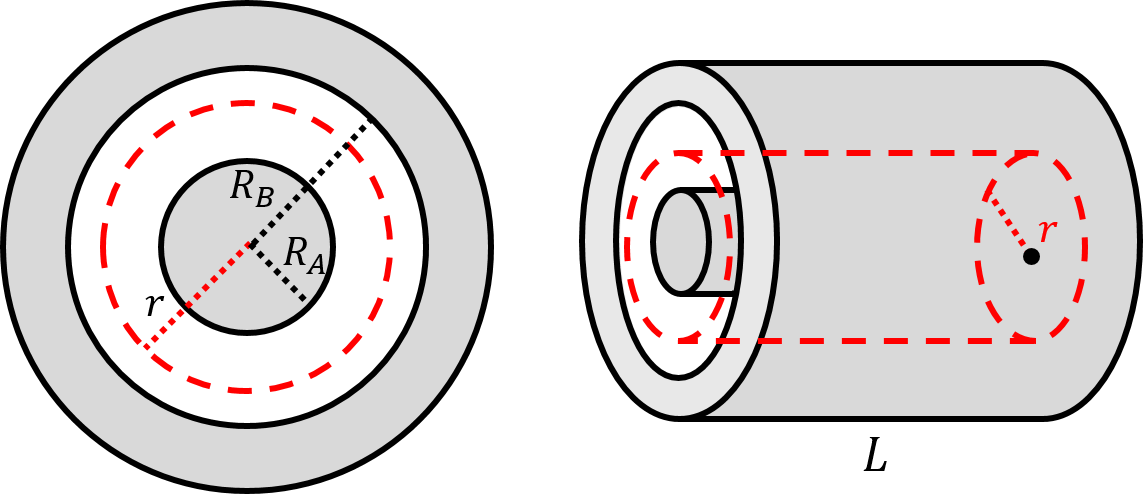
\includegraphics[width=0.7\linewidth]{files/nestedcylinderssolut-c2c6a5ac14cf1e31b82c47ac5cea4d1f.png}
\caption[]{Solving for $E$ between two cylinders using Gauss' law.}
\label{fig:potential:nestedcylinderssolution}
\end{figure}

Applying Gauss' Law:
\begin{equation}
\int E\cdot dA &= \frac{Q_{enc}}{\epsilon_0}\\
E 2\pi rL &= \frac{\lambda L}{\epsilon_0}\\
\therefore E(r) &= \frac{\lambda }{2\pi \epsilon_0 r}
\end{equation}
and the electric field points in the radial direction (outwards if the inner electrode is positive). We can find the potential difference between the two electrodes using the electric field:
\begin{equation}
\Delta V &= V(R_B)-V(R_A)= -\int_{R_A}^{R_B} \vec E \cdot d\vec r\\
&=-\int_{R_A}^{R_B} \frac{\lambda }{2\pi \epsilon_0 r} dr\\
&= -\frac{\lambda }{2\pi \epsilon_0}\ln\left( \frac{R_B}{R_A} \right)
\end{equation}
where we should note that the minus sign is ambiguous, as the actual sign of the potential difference will depend on the sign of $\lambda$, the charge on the inner cylinder. If the charge on the inner cylinder is positive, the potential difference is negative, indicating that the outer cylinder is at a lower potential than the inner one (which makes sense, as the electric field would point outwards between the two cylinders).

We can determine the capacitance between the electrodes, by taking the absolute value of the potential difference above, and using the fact that the charge, $Q$, on a length, $L$, of one electrode is given by $Q=\lambda L$:
\begin{equation}
Q &= C\Delta V\\
\lambda L &= C\frac{\lambda }{2\pi \epsilon_0}\ln\left( \frac{R_B}{R_A} \right)\\
\therefore C&=\frac{2\pi \epsilon_0}{L\ln\left( \frac{R_B}{R_A} \right)}
\end{equation}
We note that the capacitance does not depend on the (arbitrary) charge per unit length, $\lambda$ that we placed on the inner cylinder in order to model the capacitor. The capacitance only depends on the geometry of the capacitor, and the material that is used between the plates.
\end{framed}